\documentclass[a4paper, 10pt]{article}
    \usepackage[subpreambles=true]{standalone}
    \usepackage[english, american, british]{babel}
    \usepackage[utf8]{inputenc}
    \usepackage[T1]{fontenc}
    \usepackage{hyphenat}
    \hyphenation{Mathe-matik wieder-gewinnen}
    \usepackage{amsmath}
    \usepackage{import}
    \usepackage{tabularx}
    \usepackage{graphicx}
    \usepackage[margin=2cm ]{geometry}

    \title{Einführung in die Softwaretechnik 2018 \\ Sheet 05}
    \author{Maximilian Frühauf}

\begin{document}
\maketitle
\begin{enumerate}
    \item
    Explain the difference between a 3-layered architectural style and a 3-tier architecture.
    \vspace{0.5cm}

    A 3-layered architecture is a system that has 3 hierarchically ordered layers in the model.
    Each of these builds on top of the next and can be realized with an open or closed architecture.
    An example for this would be a basic GUI application where all user interaction is handled on the 
    View layer. This input is then passed on to various Controller(s) to be processed. If any of the 
    internal state of the application needs to be changed as a result, the Model layer is updated.



    A 3-tier architecture however is also divided into three separate layers, but these are then 
    distributed to three different physical systems.
    This architecture style is for example present in most modern web applications, where the first 
    tier is the user's web browser. It then connects to the application's web server and 
    receives html, css and JavaScript files. If any state needs to be saved or loaded the 
    third tier is invoked. This is the database backing the web server.
    \item
    Create a UML component diagram for Bumpers based on the following analysis object model. 
    Use the Model View Controller (MVC) architectural style and explain why you modeled it like this.
    \vspace{0.5cm}
    
    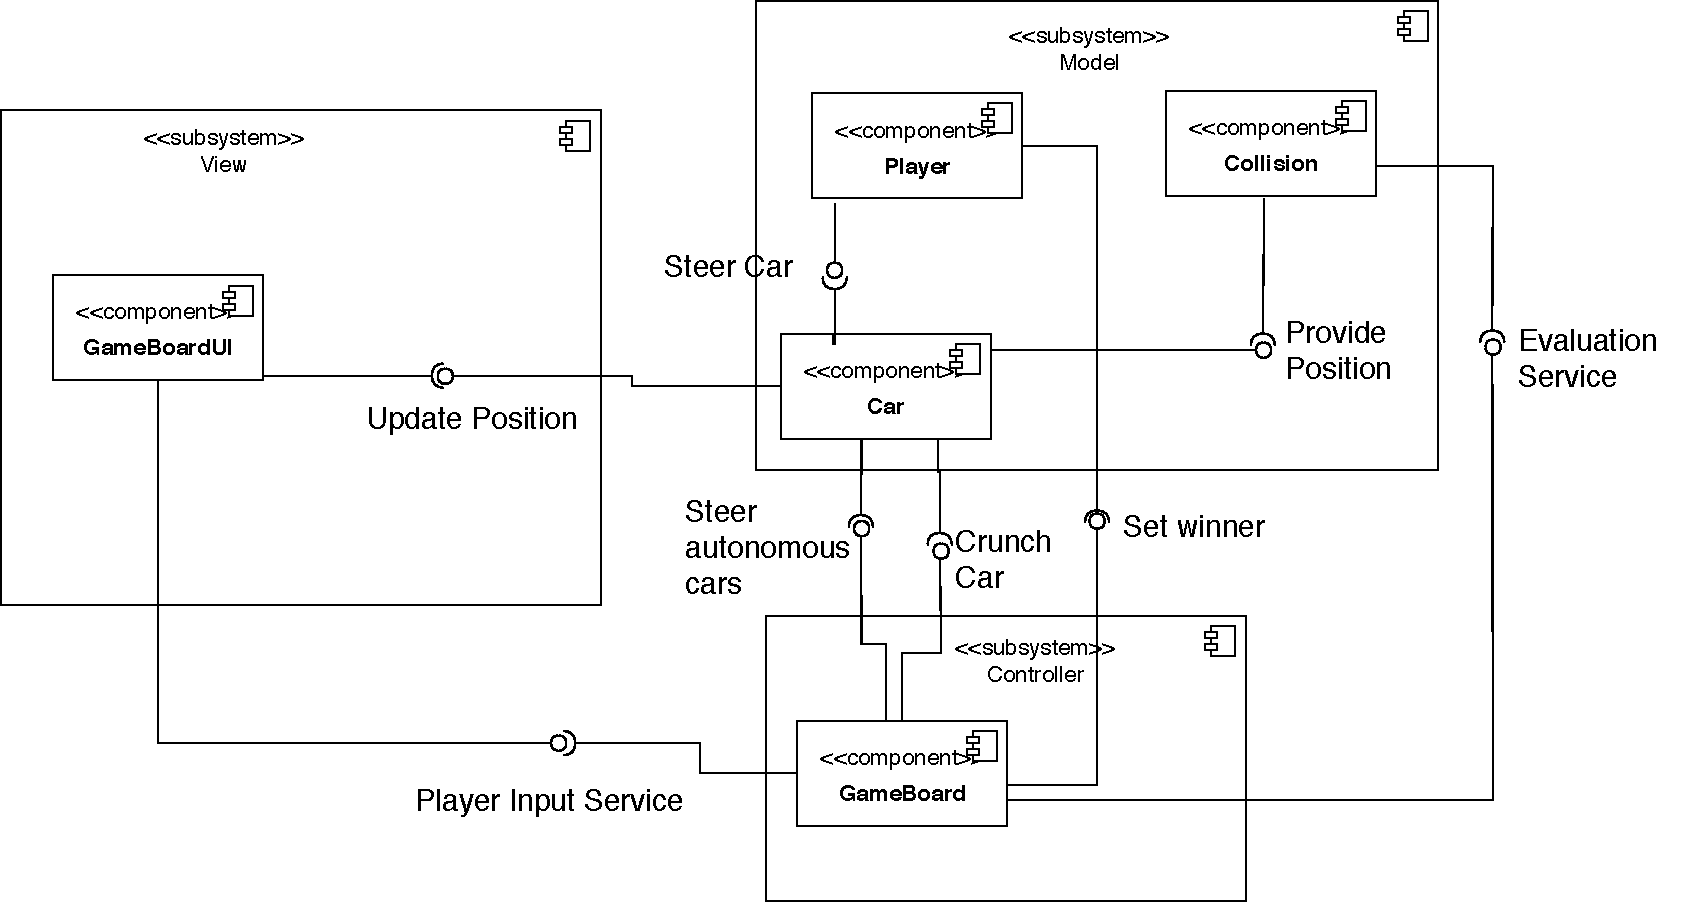
\includegraphics[width=\linewidth]{task2.pdf}

    The Model-View-Controller architectural style consists of three subsystems. The View for displaying data
    to the user, the model for holding the application state and the controller, which performs changes on
    the model.

    The inheritance hierarchies of Car and collision are modeled as a single component respectively as 
    they perform similar functionality and a component diagram is supposed to model separate logical components 
    of a system, not independent classes.The direction of the lollipop connectors is chosen as to represent the 
    data flow of the different components. A sending one is marked with the round, the receiving one with 
    the half moon ending.

    To apply this patten to the bumpers game I chose to move the GameBoardUI component to the view subsystem as
    it is responsible for displaying the changes in model state to the user. 
    Therefore it is provided the position of each of the cars via the \textit{update Position} connector by
    the car subsystem. If any of the cars position on the board changes, that change is displayed in the 
    GameBoardUI class. To be able to act on user input it provides this data via the \textit{Player Input Service} 
    to the GameBoard Component.

    The model component consists of the Player, car and collision subsystems as they both save the sate of the application
     and are therefore entity objects. 
     As the Player steers his car, it is 
     connected via the \textit{Steer Car} service to the car component. The player is also connected to the GameBoard in the
     Controller subsystem via the \textit{Set winner} service. Here the GameBoard sets the winner of the game to 
     the player if he has crushed all of the autonomous cars on the board. 
     The Collision component in the model receives the call to evaluate if a collision occurred from the GameBoard via the
     \textit{Evaluation Service}.     
     The Car component is connected to the Collision component via a \textit{Provide Position} service. Here both
    of the cars participating in a collision send their position to the Collision component.
    It is also twice connected to the GameBoard component. Here is receives data on the postions of the autonomous cars 
    via the \textit{Steer autonomous cars} service and gets data on which car to crunch as a result of a collision.

    The Controller Component just consists of the GameBoard subsystem and is responsible for mediating the communication 
    of the GameBoardUI with the Model subsystem.

    \item
    Consider the following extension to Bumpers. 
    The game includes a high- score mechanism to determine the best players. 
    High-scores are saved on a separate database server and are accessed by the game through an 
    application server. To improve redundancy, two identical database servers should be used: 
    the first acts as a main server, and the second acts as a redundant back-up in case the 
    first one fails. The Bumpers game accesses data through the application server. 
    Game administrators have the option of using a proprietary client that accesses the databases 
    directly. Draw a UML deployment diagram representing the hardware/ software mapping of this 
    system and explain why you modeled it like this. Which architectural style did you choose?
    \vspace{0.5cm}


    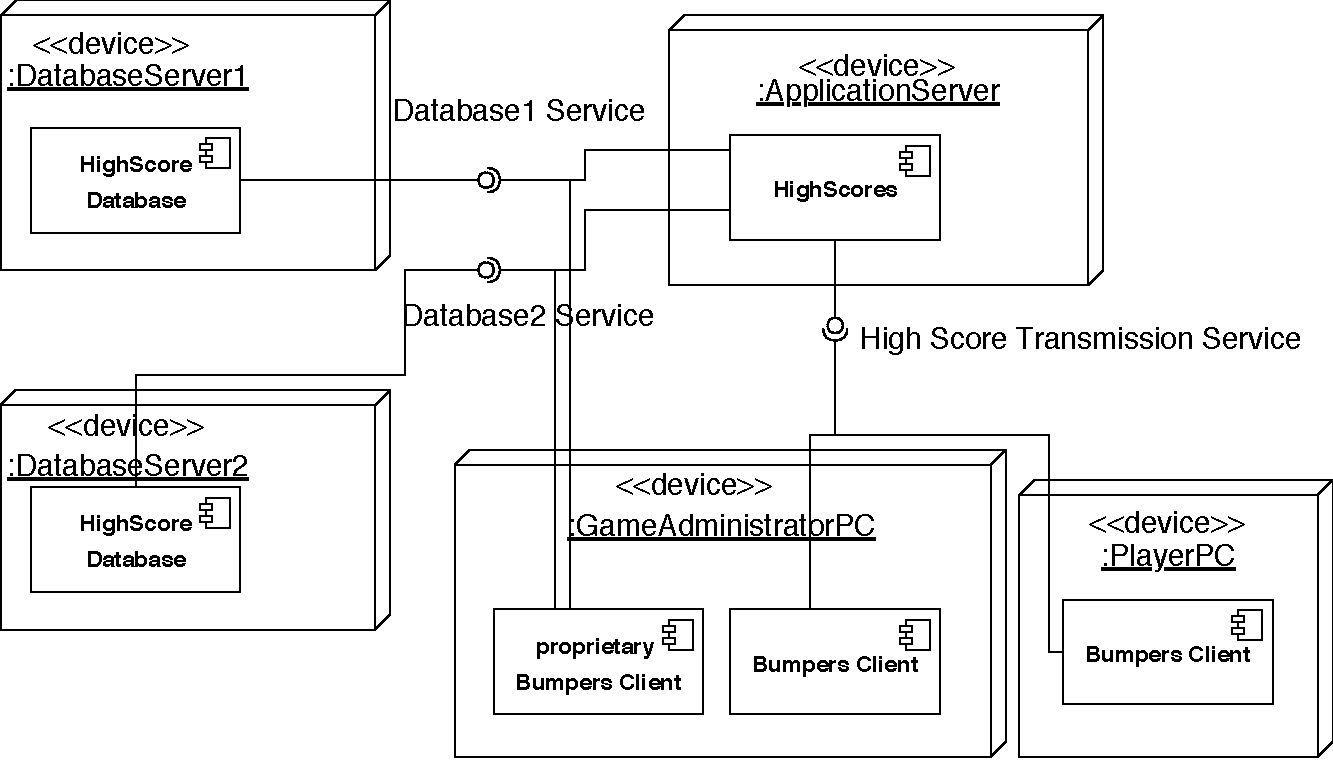
\includegraphics[width=\linewidth]{task3.pdf}


    The architectural style chosen is a 3-tiered architecture.
    Here the first tier is the \underline{:PlayerPC}. This is the interaction device of the player with the system.
    On this machine is the Bumpers Client, which connects via the \textit{High Score Transmission Service} to the
    \underline{:ApplicationServer}. This is the second tier of the architecture.

    The \underline{:ApplicationServer} then connects to both of the redundant \underline{DatabaseServer}s. 
    If one of the servers fails the other one can be used because of this architectural descision.

    Another device is the \underline{:GameAdministatorPC}. This device is running the Bumpers Client to be able to 
    experience the game as a user would for testing purposes, as well as the proprietary Bumpers Client.
    the proprietary Bumpers client to be able to acc
    \item
    Consider a legacy, fax-based, problem-reporting system for an aircraft manufacturer. 
    You are part of a reengineering project replacing the core of the system with a 
    computer-based system that includes a database and a notification system. 
    The client requires the fax to remain an entry point for problem reports. 
    You propose an E- mail entry point. Describe a subsystem decomposition that would allow 
    both interfaces. Note that such systems are used to process many problem reports per 
    day (e.g., 2000 faxes per day). Draw a UML component diagram representing the 
    subsystem decomposition of this system and explain why you modeled it like this.
    \vspace{0.5cm}

    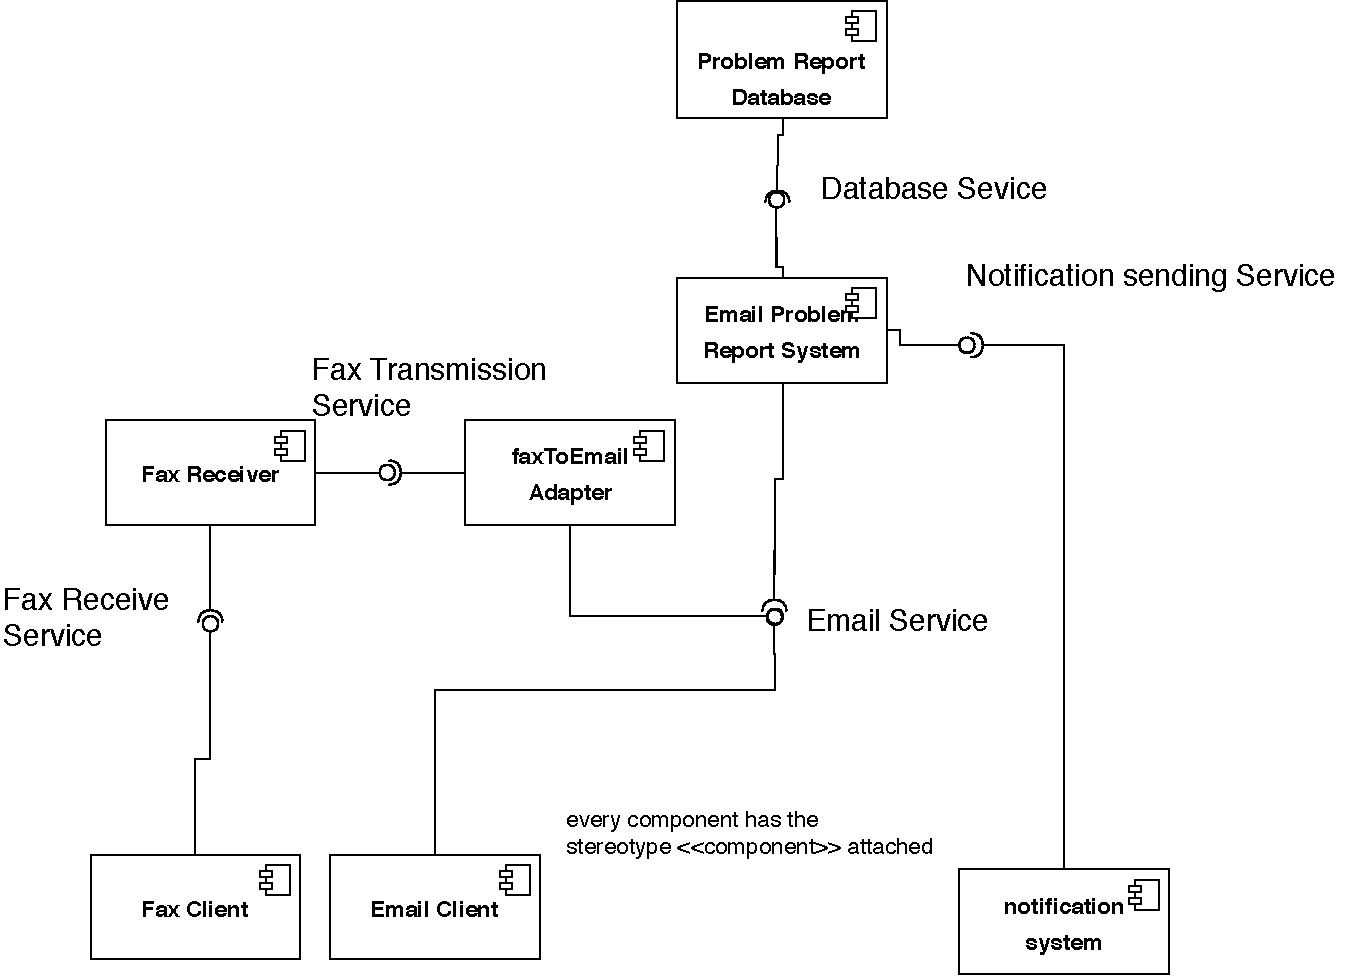
\includegraphics[width=\linewidth]{task4.pdf}

    The problem-reporting system has to endpoints that are exposed to the user. The Fax- and Email clients. 
    These are used to send reports to the system. A fax is received by the \textit{Fax Receive Service} and 
    processed by the Fax Receiver component. As the fax is the last legacy part of the system, any faxes that are 
    transmitted to it are converted to the faxToEmail adapter by the \textit{Fax Transmission Service}. Here the 
    faxes are converted to plain text.

    The plain text generated is then packaged as an email and then send via the \textit{Email Service} to the
    Email Problem Report System. Regular emails from the new Email Client are also send to via the same service.
    To make sure the system is able to process 2000 faxes and more per day, all reports are processed by the central 
    Email Problem Report System. For each of the Reports a notification is sent to the \textit{notification sending Service} 
    to the notification system which is used by the aircraft manufacturer to be able to handle the Problem reports.
    All reports handled are also sent to the Problem Report Database, where they are stored. 
\end{enumerate}
\end{document}